\documentclass[a4paper]{article}

\usepackage{amsmath}
\usepackage{physics}
\usepackage{hyperref}
\usepackage[all]{hypcap} % Make a hyperlink navigate to the top of the figure
\usepackage{graphicx}
\graphicspath{ {./images/} }
\usepackage[a4paper,left=3cm,right=3cm,top=2.5cm,bottom=2.5cm]{geometry}

\title{Quantum Fourier Transform}
\author{Tzu Hsuan Chang}

\begin{document}
\maketitle

\section{Introduction}
\label{sec:Intro}
Briefly speaking, quantum Fourier transform (QFT) is discrete Fourier transform on quantum devices.


\subsection*{Discrete Fourier Transform}
\label{subsec:dft}
DFT transform a $N$ dimension vector $x_0, x_1, ... ,x_{N-1}$ to another $N$ dimension vector $y_0, y_1, ... ,y_{N-1}$ as following,
    \begin{equation} \label{eq:eq1}
    \setlength{\jot}{10pt}
    \begin{aligned}
        \large y_k \equiv \frac{1}{\sqrt{N}} \sum_{j=0}^{N-1} x_j e^{2\pi ijk / N}.
    \end{aligned}
    \end{equation}


\subsection*{Quantum Fourier Transform}
\label{subsec:qft}
On the other hand, QFT, operates the same transformation but with different form of notation. Consider an orthonormal basis $\ket{0}, \ket{1}, ... ,\ket{N-1}$, QFT acting on this basis is defined to be
    \begin{equation} \label{eq:eq2}
    \setlength{\jot}{10pt}
    \begin{aligned}
        \ket{j} \longrightarrow \frac{1}{\sqrt{N}} \sum_{k=0}^{N-1} e^{2 \pi i j k / N} \ket{k}.
    \end{aligned}
    \end{equation}
    
Assuming $N = 2^n$, noting that we can write $\ket{k}$ into the binary form 
$\ket{k_1 \dotso k_n}$, specifically, $k = k_1 2^{n-1} + k_2 2^{n-2} + \dotso + k_n 2^0$ 
and 
$\sum_{k = 0}^{2^n-1} e^{k/2^n} \ket{k} = \sum_{k_1 = 0}^{1} \dotso \sum_{k_n = 0}^{1} e^{(\sum_{l = 1}^{n} k_l 2^{-l})} \ket{k_1 \dotso k_n}$. 
To implement QFT on quantum devices, it would be convenience to use the following representation,
    \begin{equation} \label{eq:eq3}
    \setlength{\jot}{10pt}
    \begin{aligned}
        \ket{j} &\longrightarrow \frac{1}{\sqrt{N}} \sum_{k=0}^{N-1} e^{2 \pi i j k / N} \ket{k} \\
            &= \frac{1}{2^{n/2}}   \sum_{k=0}^{2^n-1}   e^{2 \pi i j k / 2^n}   \ket{k} \\
            &= \frac{1}{2^{n/2}}    \sum_{k_1 = 0}^{1} \dotso \sum_{k_n = 0}^{1}   e^{2 \pi i j (\sum_{l=1}^{n} k_l 2^{-l})}   \ket{k_1 \dotso k_n} \\
            &= \frac{1}{2^{n/2}}    \sum_{k_1 = 0}^{1} \dotso \sum_{k_n = 0}^{1}   \bigotimes_{l = 1}^{n} \   e^{2 \pi i j k_l / 2^{-l}}   \ket{k_l} \\
            &= \frac{1}{2^{n/2}}    \bigotimes_{l = 1}^{n} \   \bigg[ \sum_{k_l = 0}^{1}   e^{2 \pi i j k_l / 2^{-l}}   \ket{k_l} \bigg] \\
            &= \frac{1}{2^{n/2}}    \bigotimes_{l = 1}^{n} \   \bigg[ \ket{0} + e^{2 \pi i j / 2^{-l}} \ket{1} \bigg] \\
            &= \frac { \big( \ket{0} + e^{2 \pi i 0.j_n} \ket{1} \big)   \big( \ket{0} + e^{2 \pi i 0.j_{n-1} j_n} \ket{1} \big)   \dotso   \big( \ket{0} + e^{2 \pi i 0.j_1 j_2 \cdots j_n} \ket{1} \big) } {2^{n/2}}.
    \end{aligned}
    \end{equation}


\section{Implementation}
\label{sec:Implement}
With the following representation
    \begin{equation} \label{eq:eq4}
    \setlength{\jot}{10pt}
    \begin{aligned}
        \ket{j_1, \cdots, j_n} &\longrightarrow   \frac { \big( \ket{0} + e^{2 \pi i 0.j_n} \ket{1} \big)   \big( \ket{0} + e^{2 \pi i 0.j_{n-1} j_n} \ket{1} \big)   \dotso   \big( \ket{0} + e^{2 \pi i 0.j_1 j_2 \cdots j_n} \ket{1} \big) } {2^{n/2}},
    \end{aligned}
    \end{equation}
we are able to construct an efficient circuit for quantum Fourier transform. To implement QFT circuit, we need the following two gates, single-qubit Hadamard gate $H$ and two-qubit controlled rotation $CROT_j$,
    \begin{equation} \label{eq:eq5}
    \setlength{\jot}{10pt}
    \begin{aligned}
        \hat{H} \ket{j}   &=   \frac{1}{\sqrt{2}}   \big( \ket{0}   +   e^{2 \pi i j/2 } \ket{1} \big), \\
        \hat{CROT_j} \ket{0j}   &=   \ket{0j}, \\
        \hat{CROT_j} \ket{1j}   &=   e^{2 \pi i j / 2^j} \ket{1j}.
    \end{aligned}
    \end{equation}
    
    \begin{figure}	
        \centering
            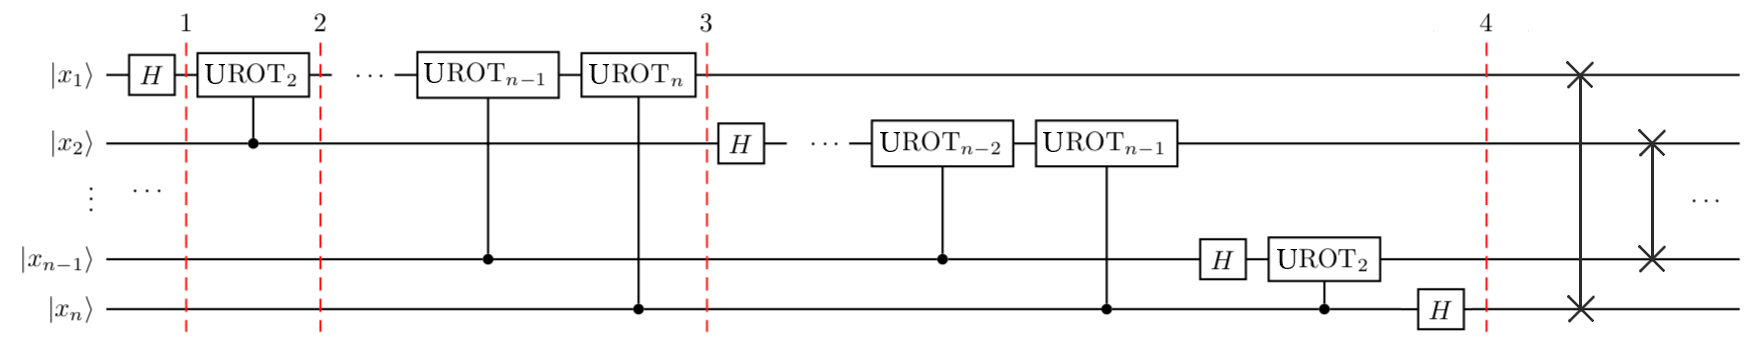
\includegraphics [width=\textwidth, height=\textheight, keepaspectratio] {qft.png}
        \caption{Quantum Fourier transform circuit.}
        \label{fig:qft}
    \end{figure}

The QFT circuit is shown on figure~\ref{fig:qft}. Please refer to the Jupyter notebook for details of the implementation example of 3 qubits quantum Fourier transform.


\end{document}